\section{FeatureSpy设计}
\label{sec:featurespy-design}
我们在设计 \sysnameF 时考虑了以下目标。

\begin{itemize}[leftmargin=*]
\item {\bf 攻击检测。} 它可靠地检测学习内容攻击以防止客户端篡改(即鲁棒性)。此外,它实现了捕获攻击的高概率,而误判的数量很少。
\item {\bf 保密性和带宽/存储效率。} 保留基于数据源的加密后重复数据删除,从而达到数据保密性和带宽/存储效率。此外,它还减轻了由于密钥泄露导致的信息泄露。
\item {\bf 低性能开销。} 它检测写入路径中的学习内容攻击,并在加密后重复数据删除部署中产生低性能开销。
\item {\bf 有限可信计算库 (TCB)。} 它管理 SGX安全区的最小信任部分和函数调用接口;鉴于滥用接口函数调用 \cite{lie05},这是一个必要的设计目标。
\end{itemize}

我们首先提出一个稻草人(不安全)设计来演示我们如何通过监控内容处理来检测学习内容攻击。然后,我们提出 \sysnameF,它可以防止恶意客户端绕过攻击检测程序。


\subsection{原型设计}
\label{subsec:featurespy-basic}
\paragraph*{Overview.} 我们的见解是,发起学习内容攻击的对手枚举了许多 {\em similar} 块,这些块遵循相同的内容模式,并在几个区域发生信息变化。换句话说,这样的块很可能共享相同的 {\em 内容特征}(可以基于相应的块内容通过 {\em N-transform} \cite{shilane12} 生成,参见后面的部分 “features本小节的提取”),并在一个小的时间窗口内进行处理。这导致攻击过程中每个时间窗口的{\em skew feature distribution},因为一些特征被一起处理的大多数块共享。

另一方面,我们认为在实际未篡改的存储工作负载中,连续块(一起处理 \cite{zhu08})的特征分布通常是 {\em uniform}(即,不同的特征对应于相同数量的块)。具体来说,我们分析了两个真实世界的数据集(有关数据集的详细信息,请参阅 \S\ref{subsec:featurespy-datasets}),并将每个数据集中的块流划分为多个不重叠的窗口,这样每个窗口都包含 $W$ 连续块。我们通过 N 变换 \cite{shilane12} 为每个块提取三个有序特征。对于每个窗口,我们计算共享相同第 i 个特征($ i=1、2$ 和 $3$)。窗口的归一化差值越小,表示对应的特征分布越均匀。


图~\ref{fig:featurespy-featureDistribution} 展示了所有窗口(大小分别为 $W$ = 1\,K, 5\,K, 和 10\,K)基于它们的第一个特征(即, $i$ = 1)。其他特征的结果是相似的,因为不同阶的特征不太可能相同(由于 N 变换原理);因此我们在这里省略它们。我们观察到,尽管不同窗口之间的归一化差异分布是倾斜的,但每个窗口只有一个小的归一化差异值(例如,Linux 中高达 0.035,CouchDB 中高达 0.005)。当$W$ = 1\,K, 5\,K 和 10\,K 时,91.5\%、58.3\% 和 29.9\% 的特征甚至被相同数量的块共享(即均匀特征分布) CouchDB 窗口,分别。

\begin{figure}
  \centering
  \begin{tabular}{cc}
    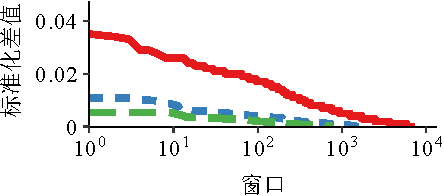
\includegraphics[width=0.45\textwidth]{pic/featurespy/plot/featureDistribution/featureDistributionLinux.pdf} &
    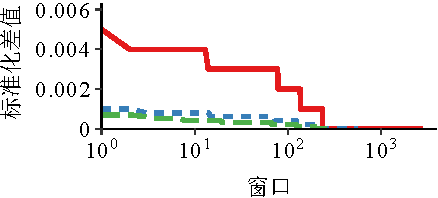
\includegraphics[width=0.45\textwidth]{pic/featurespy/plot/featureDistribution/featureDistributionCouchbase.pdf} \\
    {\small (a) Linux} & {\small (b) CouchDB} \\
    \end{tabular}
  \vspace{-6pt}
  \caption{两个真实数据集中不同窗口的标准化差异。 x 轴上的窗口按它们的归一化差异排序。}
  \label{fig:featurespy-featureDistribution}
  \vspace{-6pt}
\end{figure}

因此,稻草人设计通过 {\em 区分特征分布} 来检测学习内容攻击。图~\ref{fig:featurespy-architecture-strawman} 展示了稻草人设计的架构工作流程。由于 \sysnameF 与可能篡改未受保护内存的客户端位于同一位置,因此它通过 SGX安全区保护特征提取和攻击检测程序,从而诚实地报告攻击事件。具体来说,它进入安全区以提取每个明文块的内容特征,如果许多块匹配相同的内容特征(即相似),则报告攻击。如果没有宣布攻击,它将继续执行基于数据源的加密后重复数据删除 (\S\ref{subsec:featurespy-basics})。在下文中,我们将讨论设计细节。


\paragraph*{特征提取。}
我们通过 {\em N-transform} \cite{shilane12} 提取每个明文块的内容特征,这被广泛用于检测块级相似性。 N-transform 是基于 $N$(例如,默认为 12)对系数 $(a_i, m_i)$ 定义的,其中 $N$ 表示有多少 {\em sub-features}(基于 N-transform 生成的特征,见下文)为每个块提取。具体来说,对于每个明文块 $M$,它使用 Rabin 指纹 \cite{rabin81} 在块数据的 32 字节滑动窗口上计算许多指纹,并将每个滑动窗口中的 Rabin 指纹 $fp$ 转换为:
\begin{eqnarray}
  \label{eq:featurespy-feature}
  \pi_i = a_i * fp + m_i \mod 2^{32},
\end{eqnarray}
其中$i$ = 1, 2,\ldots, $N$。如果在其他 Rabin 指纹中,$fp$ 导致 {\em 最大值} $\pi_i$,则它将 $M$ 的第 $i$ 个子特征导出为 $fp$。基本原理是小区域的变化可能会影响一些 Rabin 指纹,其中只有少数(作为子特征)产生 $\{\pi_i\}$ 的最大值。因此,对于类似的块,大多数子特征保持稳定。

N-transform 通过将多个(例如,默认情况下为四个)连续的子特征组合在一起来计算一个特征。它通过一组特征 $S$(例如,默认情况下特征数量 $|S| = 3$)来表征每个块,以减轻比较许多子特征以进行相似性检测的计算开销。具体来说,两个块的共同特征越多,它们就越有可能相似。


\paragraph*{攻击检测。}
我们在安全区中管理一个哈希表来跟踪有多少明文块共享相同的内容特征。哈希表的每个条目将一个特征映射到该特征在不同块中出现的次数(四个字节)。此外,我们定义了一个窗口大小 $W$(例如,默认为 5\,K)并定期清除每个处理 $W$ 块的所有表条目,这样哈希表只保留 {\em 最近} 出现的特征短时间内。请注意,哈希表最多为 5\,K $\times$ 3 $\times$ (16 bytes + 4 bytes) $\approx$ 300\,KiB 并为 SGX安全区添加了可忽略的内存开销,其中每个块都有三个特征,每个特征由四个子特征拼接而成,每个子特征根据 N-transform 的默认配置占用四个字节。

为了检查每个明文块,我们根据其内容特征查询哈希表。如果一个特征不存在,我们将这个特征添加到哈希表中,并用一个初始化对应的出现;否则,如果该特征存在,我们将相应的出现加一。如果发生达到窗口大小 $W$ 的预定义比率 $T$(例如,默认情况下为 3\%),我们将报告攻击。



\subsection{FeatureSpy概览}
\label{subsec:featurespy-secure_design}

稻草人设计的一个安全限制是它容易{\em 绕过}攻击检测程序(图~\ref{fig:featurespy-architecture-strawman})。 具体来说,恶意客户端可以直接注入其自构建的块以供未受保护的操作(例如,密钥生成)处理,以发起学习内容攻击(\S\ref{subsec:featurespy-basics})。


\begin{figure}
  \centering
  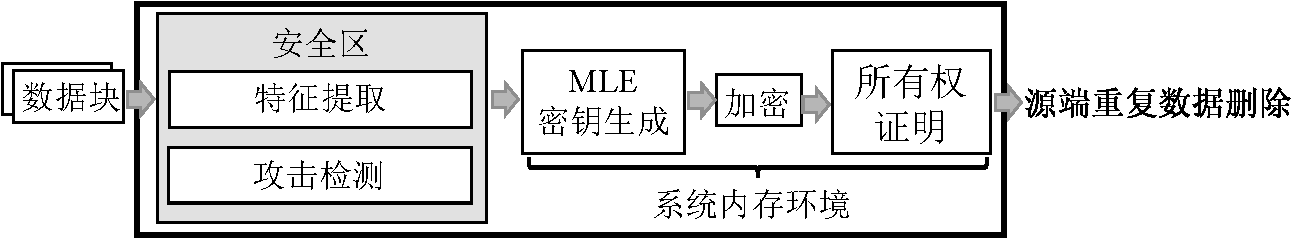
\includegraphics[width=\textwidth]{pic/featurespy/naive.pdf}
  \caption{Architectural workflows of \textit{Strawman design}. It is vulnerable to bypassing the detection procedure.}
  \label{fig:featurespy-architecture-strawman}
\end{figure}

\sysnameF 基于 {\em SGX-based PoW} \cite{ren21} 构建,以防止客户端逃避检测过程。具体来说,基于 SGX 的 PoW 方法 \cite{ren21} 将每个密文块作为输入并进入 SGX 安全区以计算密文块的指纹以及指纹的签名。只有当签名被成功验证时,云才会继续检查指纹是否对应于存储的密文块(即重复数据删除)。由于云根据 SGX安全区处理的 {\em authenticated} 指纹进行响应,因此客户端无法识别未经授权访问的块的存在。

因此,一种天真的方法是在稻草人设计中扩大 enclave,以在安全区中完全执行检测、密钥生成、加密和基于 SGX 的 PoW。在这种情况下,只有程序处理的块SGX安全区中的数据被云接受重复数据删除(由于基于 SGX 的 PoW),恶意客户端无法绕过任何程序。
然而,该方法会产生巨大的 TCB 并引入潜在的性能 \cite{arnautov16, harnik18, dinhngoc19} 和安全 \cite{lie05} 问题。

\begin{figure}
  \centering
  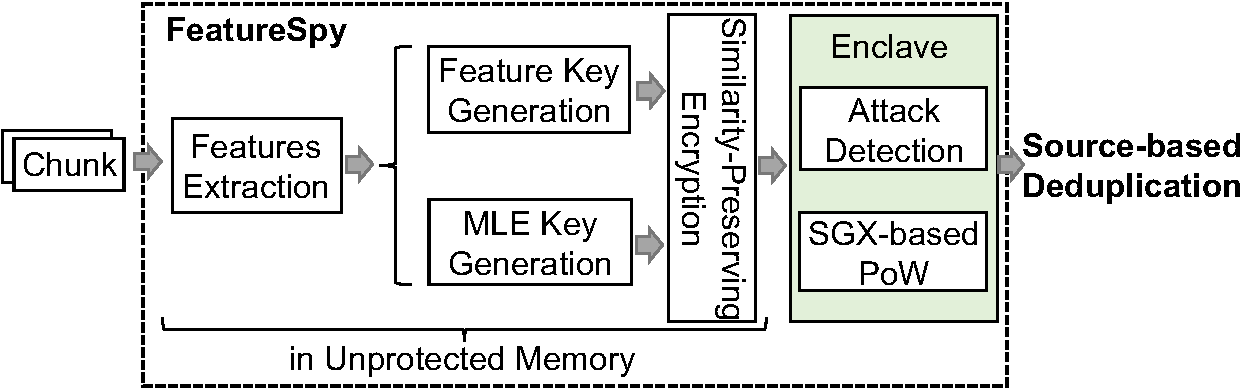
\includegraphics[width=\textwidth]{pic/featurespy/architecture.pdf}
  \caption{Architectural workflows of \textit{Secure design}. \sysnameF couples the attack detection procedure with SGX-based PoW \cite{ren21} in the enclave, in order to prevent the bypassing.}
  \label{fig:featurespy-architecture-secure}
\end{figure}

\sysnameF 提出{\em 进行基于密文块的攻击检测},并且只将检测过程与安全区中基于 SGX 的 PoW 耦合(图~\ref{fig:featurespy-architecture-secure}),以减少大小TCB 的。


\paragraph*{挑战。}
然而,{\em 基于密文块检测相似性} 提出了一个新的挑战,因为安全区现在只查看加密数据。在 MLE 之后检测相似性是不可能的,因为 MLE 密钥是从明文块 (\S\ref{subsec:featurespy-basics}) 的 {\em whole contents} 派生的。这会将相似(但不同)的明文块映射到完全不同的密文块,从而破坏相似性。

另一种加密原语是 {\em 基于特征的加密 (FBE)},它基于从每个明文块的内容特征派生的密钥(称为 {\em 特征密钥})执行加密/解密。由于相似的块仅在少数数据区域中有所不同,因此它们可能具有相同的特征密钥,以及前几个数据块(在 AES 中每个数据块占用 16 个字节)。考虑到加密后重复数据删除 \cite{douceur02, shah15} 需要一个固定的 {\em 初始化向量 (IV)}(以保持确定性加密),FBE 保持了相似块的前几个数据块的相等性(由于 {\ em block-chaining encryption} 分组密码模式的属性,例如 {\em cipher block chaining (CBC)} 和 {\em cipher feedback (CFB)} \cite{dworkin01}),并且可以通过比较进行相似性检测每个密文块中的此类数据块。


然而,FBE 容易受到密钥泄露的影响,因为一个特征密钥对应于一组具有相同内容特征的块。恶意客户端可以使用其受损的功能密钥来完全解密许多块,甚至其中一些是 {\em 超出其访问范围}。


这给选择合适的密码原语带来了两难选择:MLE 对密钥泄露具有鲁棒性(即,泄露的 MLE 密钥不能用于解密除相应的块之外的其他块)但会破坏相似性,而 FBE 保留原始块的相似性但易受攻击关键妥协。

\subsection{相似性保留加密(SPE)}
\label{subsec:featurespy-spe}

我们提出了{\em 相似性保留加密 (SPE)},它同时建立在 MLE 密钥和特征密钥之上,以通过 MLE 密钥减轻密钥泄露,同时通过特征密钥保持相似性。具体来说,由于相似块的内容差异有限,SPE 从每个明文块中抽取一小部分(例如,前 32 个字节,占 8\,KiB 块的 0.4\%),称为 {\em similarity indicator} ,使得相似块的相似度指标很可能是相同的。它用相应的特征密钥加密每个明文块的相似性指标,而剩余的大部分(占 8\,KiB 块的 99.6\%)块内容用 MLE 密钥加密。然后,我们可以通过验证相应的(加密的)相似性指标(例如,每个密文块的前 32 个字节)是否相同来检测基于密文块的相似性。请注意,SPE 不会降低跨用户加密后重复数据删除 (\S\ref{subsec:featurespy-basics}) 的存储效率,因为相同的块共享相同的内容特征(因此特征密钥)和 MLE 密钥。

我们认为 SPE 减轻了 FBE 针对密钥泄露的信息泄漏。洞察力是,受损块 $M$ 的特征密钥只能用于解密与 $M$ 相似的块的相似性指标。但是,由于此类块可能具有与 $M$ 相同的相似指标,因此 SPE 不会导致额外的信息泄漏。即使是稀有块(类似于 $M$)具有不同的相似性指标,与 FBE 相比,信息泄漏也大大减少,并受相似指标的大小影响。
在下文中,我们将介绍如何为 SPE 生成特征密钥的设计细节。


\paragraph*{功能密钥生成。}
回想一下,我们通过 N 变换(\S\ref{subsec:featurespy-basic})为每个明文块提取三个内容特征,一个基本的密钥生成方法(称为 {\tt allFeature})是连接所有特征,并计算基于连接结果的加密哈希的特征密钥。但是,{\tt allFeature} 无法为许多相似的块生成相同的特征键。具体来说,如果相似块的内容差异恰好在产生子特征(\S\ref{subsec:featurespy-basic})的滑动窗口中,则块将具有不同的特征键,并且无法检测到相似度即使剩余的原始内容相同。

我们基于 {\em 基于采样的方法} \cite{bhagwat09, dong11, qin17} 来放宽密钥生成标准。这个想法是为每个明文块采样一个{\em 代表}特征,并根据采样的特征计算特征密钥。这可以容忍内容差异,并为各种明文块生成相同的特征密钥。

我们考虑了两种选择代表性特征的方法。具体来说,{\tt firstFeature} 根据每个明文块的 {\em first} 特征生成特征密钥。优点是我们不需要计算后续的子特征和特征(\S\ref{subsec:featurespy-basic}),并减轻 N-transform 的计算开销 \cite{zhang19}。

我们还考虑 {\tt minFeature},它建立在 {\em Broder's theorem} \cite{broder97} 的基础上,根据每个的 {\em minimum} 特征(即在所有特征中具有最小值)生成特征键明文块。具体来说,布罗德定理指出,如果两个明文块具有许多共同特征(即,相似的概率很高),它们很可能共享相同的最小特征。那是:
\begin{eqnarray}
  \label{eq:featurespy-broder}
 \Pr[\min(S_1) = \min(S_2)] = \frac{|S_1 \cap S_2|}{|S_1 \cup S_2|},
\end{eqnarray}
其中 $S_i$ 是明文块 $M_i$ 的特征集合,$\min(S_i)$ 返回集合 $S_i$ ($i = 1, 2$) 中特征的最小值。因此,{\tt minFeature} 倾向于为高度相似的块生成相同的特征键。在 \S\ref{sec:featurespy-evaluation} 中,我们将研究 SPE 的不同密钥生成方法的权衡。

请注意,除了处理特征之外,另一种设计是基于第一个或最小 {\em sub-feature} 生成特征密钥。由于子特征的低熵,我们不选择这种设计。根据 N-transform 的原始配置 \cite{shilane12},每个子特征只有四个字节,攻击者可以通过枚举所有可能的子特征/密钥(最高 $2^{ 32}$)。另一方面,在 \S\ref{sec:featurespy-implementation} 中,我们重新配置 N-transform 以确保基于特征的密钥空间足够大(例如,$2^{256}$)以对抗暴力破解攻击。


\subsection{安全性分析}
\label{subsec:featurespy-security}
我们讨论了 \sysnameF 的机密性(特别是 SPE,它是底层加密原语),然后讨论了它对恶意客户端的鲁棒性。

\paragraph*{对受损云的保密性。}
我们已经讨论了 SPE 在密钥被泄露 (\S\ref{subsec:featurespy-spe}) 时相对于 FBE 的安全性改进,现在关注密钥保持安全的情况。我们的目标是证明 SPE 可以保护加密后重复数据删除对受损云的安全性。具体来说,由于 SPE 通过 MLE 和 FBE 执行加密,因此其安全性降低到 MLE 和 FBE 的安全性。之前的工作 \cite{bellare2013MLE} 表明,当明文块是从一个大的空间使得很难预测从空间中选择的任何块(即 {\em 不可预测})。在下文中,我们(非正式地)表明,如果特征不可预测,FBE 会保留 MLE 的安全性。


我们将 FBE 视为 MLE 的一种通用形式。如果我们将采样的特征(例如,{\tt firstFeature} 和 {\tt minFeature} 的代表特征,以及 {\tt allFeature} 的所有特征)视为消息 $M$,那么 FBE 实际上使用$M$的密码散列来加密对应的扩展$f(M)$(即明文块),其中$f(\cdot)$是一个扩展函数。由于每个 $M$ 都是不可预测的,因此密钥对多项式时间的对手保持机密。然后,如果底层对称加密是安全的,则对手无法区分密文和随机值。

请注意,我们的非正式分析依赖于特征不可预测的安全假设,而我们可以通过服务器辅助密钥生成 \cite{bellare13b} 来缓解不可预测的假设(请参阅 \S\ref{sec:featurespy-implementation} 了解我们如何部署 \ sysnameF 在解决不可预测假设的现有加密后重复数据删除系统中)。


\paragraph*{对恶意客户端的鲁棒性。}
我们已经讨论过攻击者无法绕过检测程序(\S\ref{subsec:featurespy-secure_design}),现在关注对其他恶意行为的鲁棒性(\S\ref{sec:featurespy-setting})。


\begin{itemize}[leftmargin=*]
  \item {\bf 案例 1:篡改不受保护的程序。}
    \sysnameF 通过 SGX 保护检测程序,但恶意客户端可以篡改未受保护的程序。它可能会操纵特征、相似性指标和密钥,以欺骗 \sysnameF。
    我们认为,这些操作无助于从遵循我们设计的其他诚实客户那里学习内容,因为这些操作导致与 SPE(由诚实客户应用)产生的密文块不同,即使原始明文块是相同的。这个 {\em 禁止重复数据删除},依赖重复数据删除模式泄漏的学习内容攻击是不可能的。
  \item {\bf 案例2:篡改数据处理。}
    由于 \sysnameF 在每个处理窗口的粒度上监控数据相似性,恶意客户端可能会篡改正在处理的数据流,并小心地插入相似的块(用于攻击),使得每个窗口只包含一小部分相似的块.尽管 \sysnameF 在这种情况下无法检测到攻击,但我们认为它减缓了学习内容攻击。例如,在没有 \sysnameF 的情况下,恶意客户端可以用相似的块(即,数量为 $W$)填充每个窗口以进行攻击,但 \sysnameF 确保它可以提交最多 $W\times T$ 的相似块(否则会被检测到)。攻击成本降低$1/T$倍。通过配置一个小的$T$,我们可以使学习内容攻击成本太高而变得不切实际;权衡是增加了误判的可能性(即在正常情况下报告攻击)。
\end{itemize}
  
  
  
  \paragraph*{限制。}
  \sysnameF 检测来自每个 {\em 独立} 客户端的学习内容攻击。但是,攻击者可能会破坏多个客户端以合作发起学习内容攻击。现在每个客户端上传的相似块的数量大大减少,\sysnameF 可能无法有效检测到异常。我们将防御合作学习内容攻击作为我们未来的工作。